\section{The Data}
\label{sec:data}
The data consists of 8675 rows of text, each with 50 posts or comments including the MBTI type of said person. It has been scraped from the "Personality Cafe forum"\footnote{http://personalitycafe.com/forum/} and made publicly available\footnote{https://www.kaggle.com/datasnaek/mbti-type}. The forum is used and maintained by personality enthusiasts which is why the users provide their MBTI type as part of their profile and thus allow for correctly labeled data.\\
The different personality types are distributed unevenly in the data, see figure \ref{fig:Hist}. Therefore, this analysis includes a model without types that occurred less than half of the expected rate for 16 personality types $\frac{1}{16 * 2}$, 3.1\% or 271 observations. This more robust model uses 7 out of 16 personality types for a more stable estimate. The most frequent personality type INFP occurs in 21\% of all cases, giving a prediction baseline of 21\% to beat.\\
There are 3 times more introverts than extraverts on the platform. This matches the notion of introverts sharing their thoughts more often online than face-to-face \cite{goby_personality_2006} though extraverts might provide the longer texts or the more frequent communication \cite{seidman_self-presentation_2013}. Sensing people also seem to be rare, of all 8 sensing personality types, only 2 types exceed the threshold for the more robust model. Hence, this adds to critical literature regarding this the sensing/intuition dimension \cite{boyle_myers-briggs_1995}.

\begin{figure}
\centering
  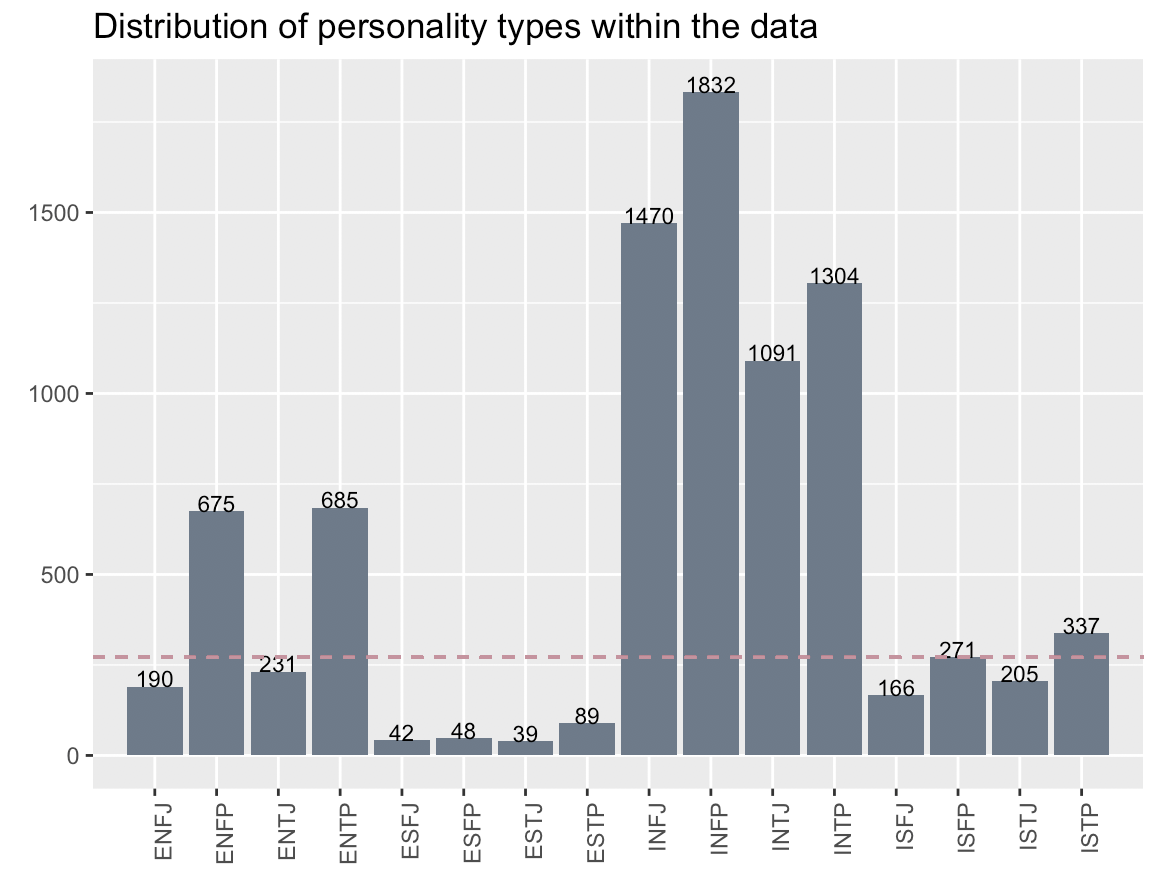
\includegraphics[scale=0.4]{histogram.png}
\caption{Histogram of all personality types including a threshold to indicate types that occurred less than half of the expected times.}
\label{fig:Hist}
\end{figure}

Though the posts rarely contain ``me as an INFP [or any other type]", the posters tend to stay within their own communities  of personality types. This leads to statements such as the following:

\begin{quote}
    ``I think the easiest and most efficient approach is a tarp, jigsaw, and mulcher. But that's just my personal preference. Not all ENTJs are the same." (ENTJ)\\[4pt]
    ``Hey @MsBossyPants are you down for a debate on Ayn Rand vs Marx? Maybe we should talk about our poor Fi? Oh I know- let's try to correlate testing ENTJ with being sociopathic.  :laughing:" (ENTJ)\\[4pt]
    ``The last thing my INFJ friend posted on his facebook before committing suicide the next day. Rest in peace~   http://vimeo.com/22842206" (INFJ)\\[4pt]
    ``a pokemon world  an infj society  everyone becomes an optimist" (INFJ)
\end{quote}

Though the users do not refer to themselves when mentioning the type, they talk about their own personality type much more often than about others, see figure \ref{fig:types}. As this might bias the performance of the model, an unbiased version of the model is included as well. Mentioning one's own personality type and staying within a community of one's own type will however be taken as an important feature for classifying one's personality since it also allows the use of networks for personality prediction.

\begin{figure}
\centering
  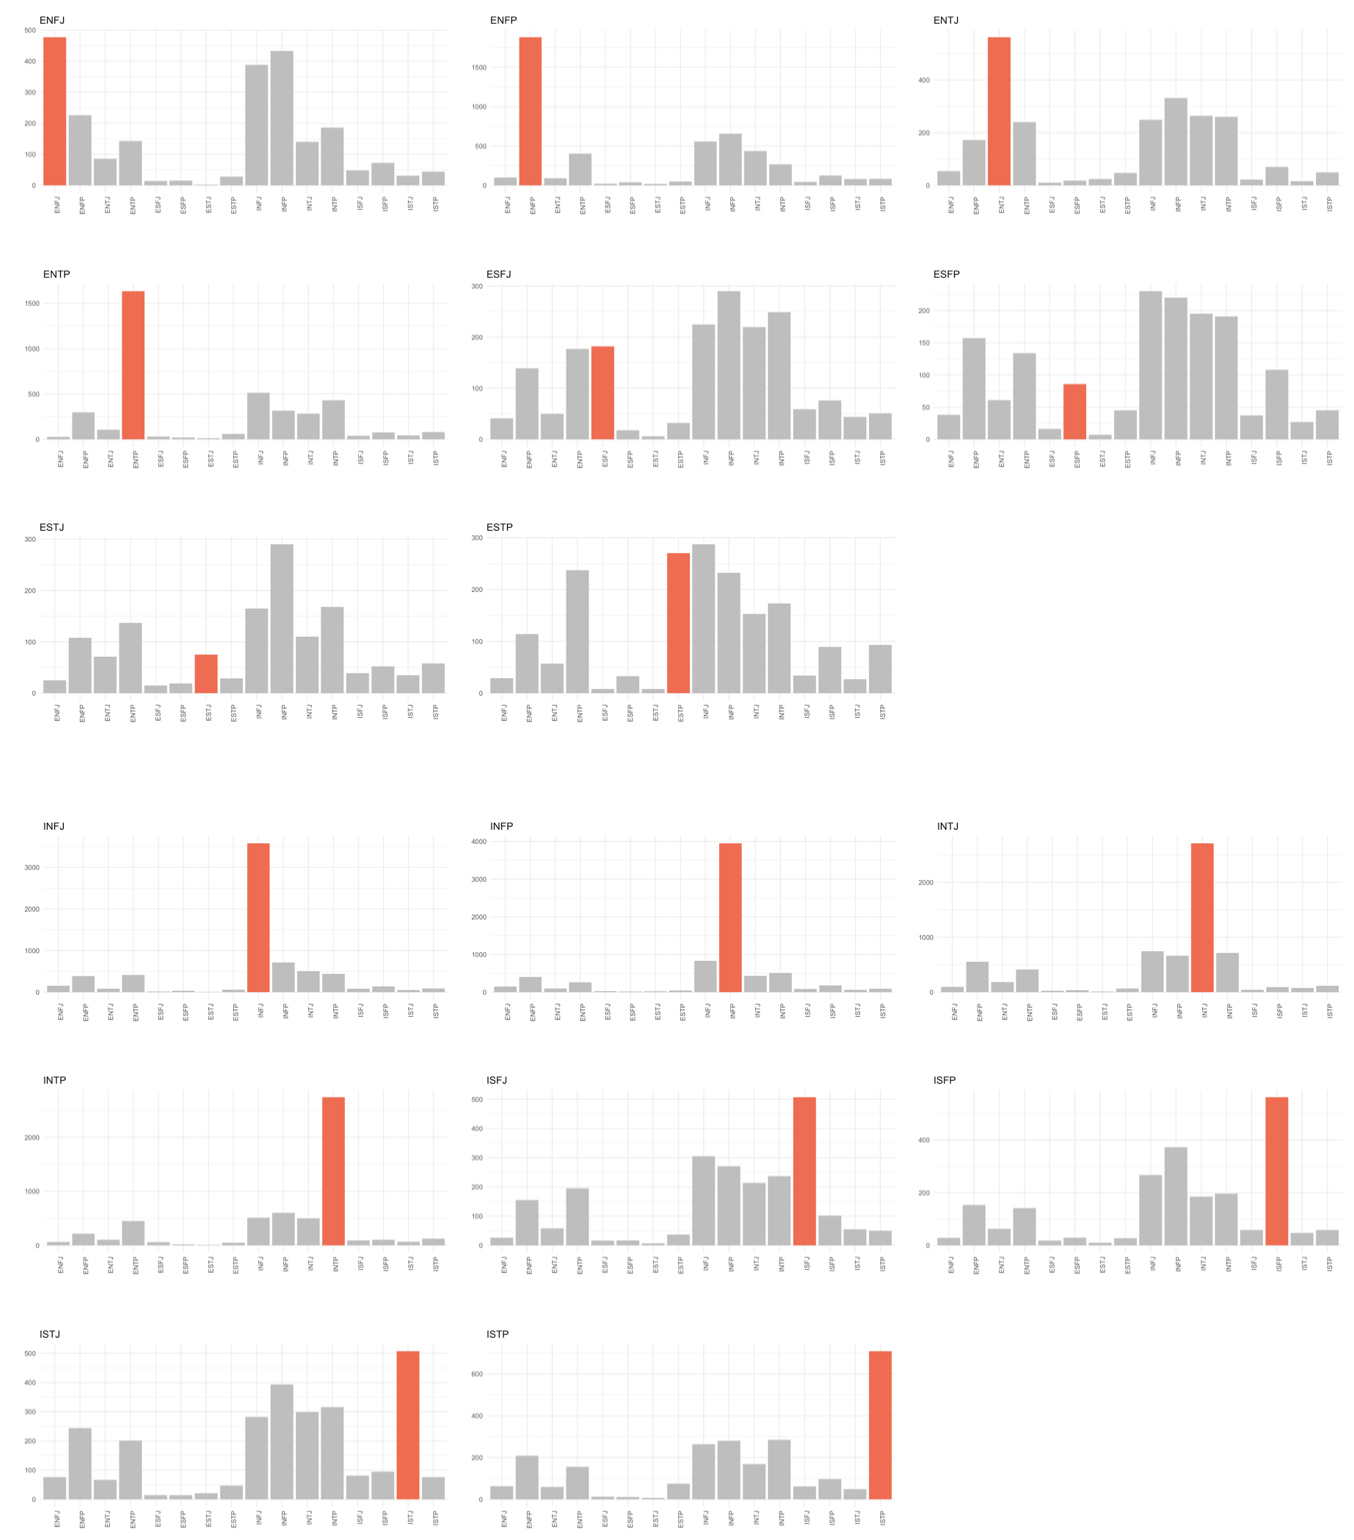
\includegraphics[width=\textwidth]{barchartstype.png}
\caption{Histograms of mentioning any personality type for each of the 16 types.} 
\label{fig:types}
\end{figure}